%%%%%%%%%%%%%%%%%%%%%%%%%%%%%%%%%%%%%%%%%%%%%%%%%%%%%%%%%%%%%%
%% LaTeX template for the science justification to be       %%
%%     submitted as part of a regular ALMA proposal.        %%
%% This template should also be used for a ToO, DDT, or     %%
%%     mm-VLBI ALMA proposal, but NOT for Large Programs    %%
%%     (these have a separate template with more sections)  %%
%%                                                          %%
%%                      ALMA Cycle 9                        %%
%%                                                          %%
%%%%%%%%%%%%%%%%%%%%%%%%%%%%%%%%%%%%%%%%%%%%%%%%%%%%%%%%%%%%%%

%%%%%%%%%%%%%%%%%%%%%%%%%%%%%%%%%%%%%%%%%%%%%%%%%%
%%%%% How to convert this document to PDF %%%%%%%%
%%%%%%%%%%%%%%%%%%%%%%%%%%%%%%%%%%%%%%%%%%%%%%%%%%

% If your figures are stored as PostScript files, you can use the 
% following commands to generate a PDF file of your proposal:

%% latex file.tex
%% dvips file.dvi
%% ps2pdf file.ps file.pdf 


% If your figures are PDF images or bitmap pictures in PNG, JPG, or GIF format,
% you can use the pdflatex command to generate a PDF file from this template
% (note, however, that the pdflatex command does not handle PostScript files):

% pdflatex file.tex

% Warnings: 
%           1. You must make sure that PDF output generated from this
%              template is complete both when displayed with a viewer 
%              (acroread, for example) and when printed on paper.
%              LaTeX installations vary greatly and therefore it might 
%              not be possible to get all proposals to come out 
%              correctly with a single text page layout. 
%              In some cases you will have to adjust the 
%              \topmargin=-7mm command in the template to center the 
%              text vertically in the page.  
%           2. The scientific justification, figures, tables, references,
%              and public outreach statement must all fit within the
%              4-page limit.
%           3. You are free to include colour images in your proposal justification.
%              Proposals are distributed to ALMA Review Panels and to distributed
%              peer review reviewers in electronic form.
%              However, the scientific content of the images should still remain
%              clear when displayed or printed in black and white.
%           4. This template is for regular, ToO, DDT, or mm-VLBI ALMA proposals,
%              but NOT for Large Programs: these have a separate template with
%              more sections, and is available from the ALMA Science Portal


%%%%%%%%%%%%%%%%%%%%%%%%%%%%%%%%%%%%%%%%%%%%%%
%%%%% Default format: 12pt single column %%%%%
%% 12pt is the minimum font size allowed !! %%
%% This applies to everything, including    %%
%% references, figure captions, and tables  %%
%% ==> Proposals not compliant to this will %%
%%     be rejected. See Section 5.3.1 in    %%
%%     the ALMA Proposer's Guide            %%
%%%%%%%%%%%%%%%%%%%%%%%%%%%%%%%%%%%%%%%%%%%%%%

\documentclass[12pt,a4paper]{article}  %% DO NOT CHANGE to 11pt or less !

\usepackage[dvipdfmx]{graphics, graphicx}
% if you on overleaf...
\usepackage{color}
% if you on local...
% \usepackage[dvipdfmx]{color}
\usepackage{amsmath,amssymb}
\usepackage{natbib}
\usepackage{aas_macros}
\usepackage{compactbib}
\usepackage{txfonts}
\usepackage{threeparttable}
\usepackage{xspace}
\usepackage[colorlinks=true,citecolor=blue]{hyperref}

\newcommand{\ammonia}{NH$_3$\xspace}

%%%%%%%%%%%%%%%%%%%%%%%%%%%%
%%%%%% Page dimensions %%%%%
%%%%%%  DO NOT CHANGE  %%%%%
%%%%%%%%%%%%%%%%%%%%%%%%%%%%

\textheight=247mm
\textwidth=180mm
\topmargin=-7mm
\oddsidemargin=-10mm
\evensidemargin=-10mm
\parindent 10pt

%%%%%%%%%%%%%%%%%%%%%%%%%%%%%
%%%%% Start of document %%%%% 
%%%%%%%%%%%%%%%%%%%%%%%%%%%%%

\begin{document}
\pagestyle{plain}
\pagenumbering{arabic}
 
% The title, abstract and list of investigators should NOT be included in the
% Scientific justification. The title and abstract are put automatically on the cover page.

%%%%%%%%%%%%%%%%%%%%%%%%%%%%%%%%%%%%%%%%%
%%%%% Body of science justification %%%%%
%%%%%%%%%%%%%%%%%%%%%%%%%%%%%%%%%%%%%%%%%

%% ENTER TEXT, FIGURES AND TABLES BELOW
%% Minimum font size for all text, references, figure captions, and tables is 12pt
%% Proposals not compliant to this will be rejected. See Section 5.3.1 in the ALMA Proposer's Guide.

\section{Scientific Justification}
% Nitrogen is the fifth most abundant elements in the interstellar medium (ISM) with elemental abundances of $\sim6\times10^{-5}$ with respect to hydrogen. 
\noindent \textbf{Background -- Nitrogen chemistry} \quad Nitrogen is one of the key elements for the chemistry of star and planet formation. It is the third most abundant heavy element after carbon and oxygen \citep{Przybilla08}. Nitrogen in star-forming clouds is incorporated into planet-forming disks as volatiles such as N$_2$, which also affects disk chemistry \citep[e.g.,][]{Schwarz14}. These volatiles eventually become the building material of planetary bodies. In addition, organics such as \ammonia that formed in molecular clouds or cloud cores set the initial condition of organic chemistry and its abundance will effectively limit the formation paths and efficiencies of nitrogen-bearing complex organic molecules in the later stages of star and planet formation.

\smallskip
\noindent Nitrogen chemistry in the interstellar medium (ISM) consists of three competing processes; conversion from N atoms into N$_2$ molecules via gas-phase reactions, the reverse process (e.g., photodissociation), and the freeze-out of N and N$_2$ onto dust grains followed by surface reactions \citep[e.g.,][]{Daranlot12}. Thus, it is expected that the main nitrogen reservoir is either in molecular (N$_2$) or atomic (N) form, or icy nitrogen-bearing molecules (e.g., \ammonia). 

\smallskip
\noindent However, the main nitrogen reservoir is not yet directly proven or inconclusive. Ice observations with \textit{Spitzer} revealed that $\sim$10\% of overall nitrogen is locked up into ices as \ammonia, NH$_4^+$, and OCN$^-$ \citep{Oberg11}. Direct observations of N and N$_2$ are difficult in both ice and gas. \citet{Maret06} instead observed N$_2$H$^+$, which is primary formed by N$_2$ + H$_3^+$, to conclude that it is unlikely that the gaseous N$_2$ is the main nitrogen reservoir. Alternatively, a large fraction of N$_2$ might be locked up into ices. A very uncertain upper limit of N$_2$ ice abundance in molecular clouds have been inferred indirectly to be $\lesssim$40\% of overall nitrogen \citep{Boogert15}. Furthermore, in situ measurements on the comet 67P/Churyumov-Gerasimenko by the Rosetta mission suggested that a substantial amount of nitrogen is hidden as ammonium salts \citep{Altwegg20}.

\medskip
\noindent \textbf{Deuteration of \ammonia ice} \quad  It is well established that deuterium enrichment is sensitive to various physical and chemical conditions and thus used to probe the formation stage of molecules \citep[e.g.,][]{Ceccarelli14}. \citet{Furuya18} proposed a new approach to constrain the main nitrogen reservoir using multiply-deuterated ammonia ice. The ammonia ice, NX$_3$, where X is H or D, are mainly formed by sequential hydrogenation of \textit{atomic N} on the dust grain surfaces in molecular clouds or dense cores. In molecular clouds, their relatively high temperature ($\gtrsim$20\,K) and low density ($\sim$10$^3$--10$^4$\,cm$^{-3}$) will result in a low D/H ratio, while it will be higher in dense cores (or prestellar cores) due to their cold ($\lesssim$20\,K) and dense ($\gtrsim$10$^5$\,cm$^{-3}$) environment and the freeze-out of CO. In particular, the D/H ratios of multiply-deuterated ammonia ices (ND$_3$/NHD$_2$ and NHD$_2$/NH$_2$D) selectively reflect the deuteration in dense cores over the NH$_2$D/NH$_3$ ratio. Thus, if the atomic N (ingredient of \ammonia ice) is the main nitrogen reservoir and \ammonia ices are mainly formed in dense cores, the D/H ratio of ammonia ices will be high (a few percent or higher) and the ratios such as [ND$_3$/NHD$_2$]/[NHD$_2$/NH$_2$D] and [NHD$_2$/NH$_2$D]/[NH$_2$D/NH$_3$] are close to the statistical value (1/3) and lower than unity. On the other hand, if the atomic N is largely converted into the stable molecular form (i.e., N$_2$ and NH$_3$) in molecular clouds, the ratios should be larger than unity. 

\begin{figure}[th]
    \centering
    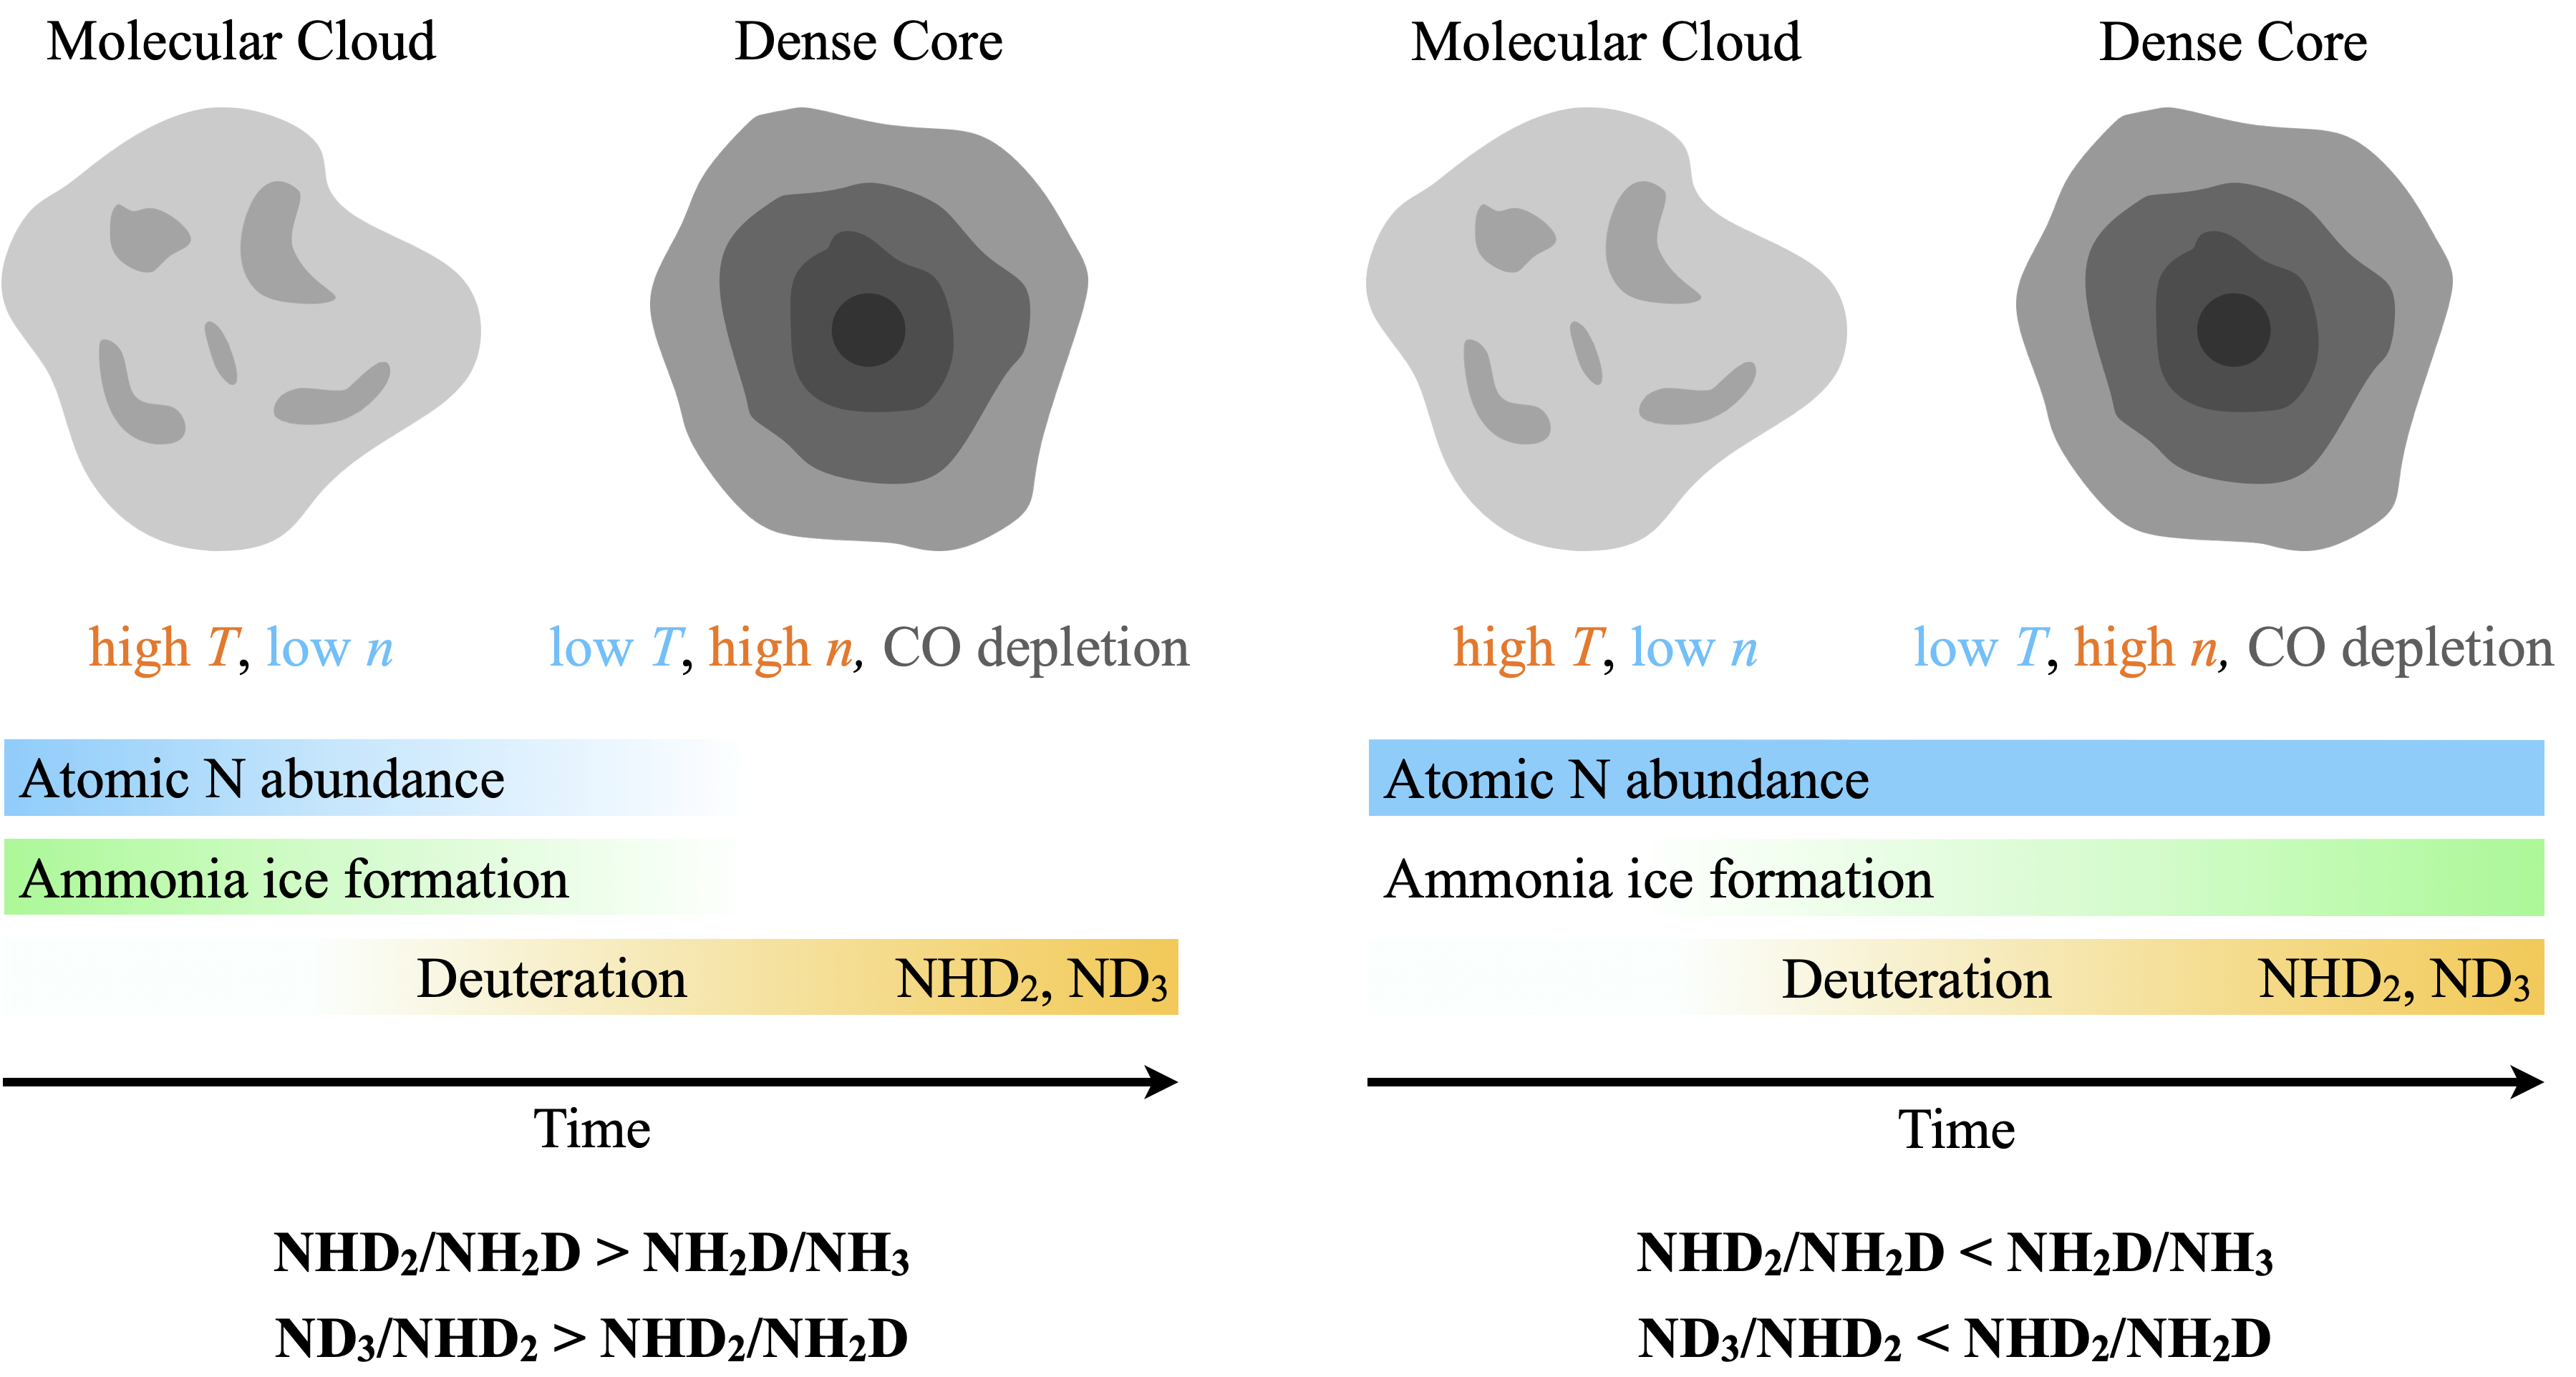
\includegraphics[width=\textwidth]{ammonia_deuteration_cartoon.png}
    \caption{Relation between the main nitrogen reservoir and deuteration of ammonia ices. left: In the case that the atomic nitrogen has been mostly converted into molecules in dense cores. This will result in the [ND$_3$/NHD$_2$]/[NHD$_2$/NH$_2$D] and [NHD$_2$/NH$_2$D]/[NH$_2$D/NH$_3$] ratios of higher than unity. right: In the case that the atomic nitrogen is remains as the main nitrogen reservoir in dense cores. The [ND$_3$/NHD$_2$]/[NHD$_2$/NH$_2$D] and [NHD$_2$/NH$_2$D]/[NH$_2$D/NH$_3$] ratios will show the statistical values and will be lower than unity.}
    \label{fig:my_label}
\end{figure}

\smallskip
\noindent The best and only way to measure the D/H ratios of ammonia ices is to observe the flesh gas that have just sublimated from the dust grain surfaces in the inner warm ($T\gtrsim100$\,K) region of the protostellar envelopes, so-called \textit{hot corinos}. \textbf{Here, we propose to observe NH$_2$D, NHD$_2$, and ND$_3$ molecular lines at $\sim$300\,GHz to measure the D/H ratios of ammoia ices toward multiple hot corinos, taking advantage of the high resolution and high sensitivity of ALMA. This will reveal the main nitrogen reservoir in star-forming clouds and will be the crucial first step to elucidate nitrogen chemistry in the ISM.}


% due to the difficulty of direct observations of N and N$_2$ in dense clouds. 



\color{red}
Introduction: Importance of nitrogen chemistry, and it is not yet elucidated, deuteration of ammonia ice can trace the ice formation history and nitrogen partitioning...

Furuya+18 proposed that the ice formation history and information about main nitrogen reservoir are imprinted into the multiply deuterated ammonia ices. [NHD2/NH2D]/[NH2D/NH3] reflects the deuteration levels of different evolutionary stages. Non-statistical ratio of [D2O/HDO]/[HDO/H2O] is explained by the scenario that the H2O ices are formed in the ealier stages mainly and the formation efficiency is reduced in the later dense core stage

We can measure the ice deuteration by observing the hot gas sublimated from dust grain surface in the vicinity of the protostar (hot corino)

We already constrained the NH2D/NH3 ratio with VLA toward prototypical hot corino IRAS 4A. High ratio suggests NH3 ice formed in the later dense core and main nitrogen reservoir could be mostly atomic N toward IRAS 4A. 

However, we need multiply deuterated ammonia to confirm the scenario proposed in Yamato et al. i.e., how is the ND3/NHD2 ratio which will better trace the later stage ice formation? Also, we need additional sources to confirm if this scenario is ubiquitous or not.

\color{black}



% ALMA uses two systems to review the proposals submitted in the Main Call.
% All proposals requesting less than 50 h on the 12-m Array and all ACA stand-alone proposals requesting less
% than 150 h on the 7-m Array will be reviewed by Distributed peer review (see Section 1.2.1 of the Proposer's Guide).
% All Large Programs will be reviewed by Panels. 
% Additionally, both systems will follow a dual-anonymous procedure, in which the proposers do not know
% who are the reviewers and the reviews do not who are the proposers.
%
% Please refer to the guidelines before writing your proposal:
%     https://almascience.org/proposing/alma-proposal-review/dual-anonymous
%
% In the following part, describe the scientific background of the project,
% pertinent references and previous work relevant to this 
% proposal, together with any figures and tables that you judge necessary
% (use the following two examples as templates, or remove)
% Please do not disclose the name(s) of the proposer(s), and write the proposal in a way
% such that the proposer(s) cannot be identified. 
 
%-----------------------------Figure Start---------------------------

% The 'scale' parameter below allows you to scale the figure so that it fits within the page.
% In this case the figure was scaled to 20% of its original size.
% Note: for .png files one has to use pdflatex, not classic latex
%
% Minimum font size for references: 12pt 
% Proposals not compliant to this will be rejected. See Section 5.3.1 in the ALMA Proposer's Guide.

% \begin{figure}[tbh]
% \includegraphics[scale=0.2]{HL_tau.jpg}
% \caption{\em{ALMA image of the protoplanetary disc surrounding the young star HL Tauri.}}
% \end{figure}
%-----------------------------Figure End------------------------------

%-----------------------------Table Start-----------------------------

% Minimum font size for references: 12pt 
% Proposals not compliant to this will be rejected. See Section 5.3.1 in the ALMA Proposer's Guide.

\begin{table}[tbh]
\begin{center}
\caption[]{\em{Here we show the continuum sensitivity required per band.}}
\begin{tabular}{cc}
\hline \noalign {\smallskip}
Frequency (GHz) & Sensitivity (mJy) \\
\hline \noalign {\smallskip}
300 & 0.10 \\
850 & 0.50 \\
\hline \noalign {\smallskip}
\end{tabular}
\end{center}
\end{table}
%-----------------------------Table End ------------------------------

\section{Description of observations}

% Please describe the observations to be made and their specific
% purpose, with a clear explanation of the need for, and 
% appropriateness of, ALMA Cycle 9 data.  


\section*{References}
\bibliographystyle{aas_compactbib}
\bibliography{reference}


%%%%%%%%%%%%%%%%%%%%%%%%%%%
%%%%% End of document %%%%%
%%%%%%%%%%%%%%%%%%%%%%%%%%%

\end{document}

